\begin{bibunit}[IEEEtran.bst]

\clearemptydoublepage
\chapter{Problem formulation and Ontology of approaches}
\label{chap:1}

\section{Problem formulation}
  \label{sec:chap1_problem_form}
We're interested in a broad class of problem that consists in finding the best function $f$ that maps available inputs $y$ to desired outputs $u$.

In geoscience $u$ and $v$ can generally be defined as $D_u$ and $D_y$ dimensional vector fields defined on spatio-temporal domains $\Omega_u$ and $\Omega_y$.
We consider here scalar fields and discrete fields as particular case of this generic formulation.
The different problems can then characterized by the type of quantities $u$ and $y$ and by the spatio-temporal domain $\Omega_u$ and $\Omega_y$ on which they are defined.
  We illustrate in Figure \ref{fig:planet_drawings} how our two use cases of sensor calibration and SSH mapping easily fit in such formulation.
  Additionnally we show in Figure \ref{fig:task_ontology} how tasks such as calibration, mapping and forecast can be seen to only differ through the domain of definition of $u$ and $y$.

\begin{figure}[htbp]
   \begin{center}
     \begin{tabular}[c]
      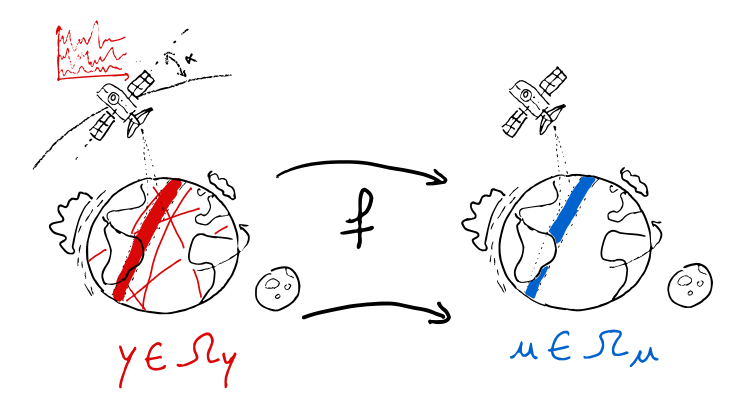
\includegraphics[width=0.8\linewidth]{Chapitre1/Ch1-Figures/Cal_drawing.png} \\
      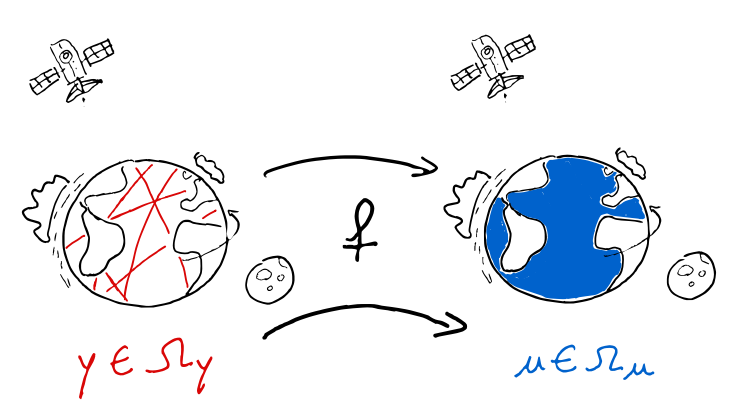
\includegraphics[width=0.8\linewidth]{Chapitre1/Ch1-Figures/Mapping_drawing.png} \\
     \end{tabular}
   \end{center}
   \caption[Swot calibration and altimetry mapping problem illustration]
     {\footnotesize The calibration problem (top row) consists in finding the mapping $f$ that estimates the observed SSH $u$ from the SWOT satellite given the actual noisy measurement and ancillary calibrated measures ($y$). 
     The mapping task (bottom row) consist in finding an operator $f$ that maps partial measurements of the SSH $y$ to a map of SSH $u$}
   \label{fig:planet_drawings}
\end{figure}

\begin{figure}[htbp]
   \begin{center}
      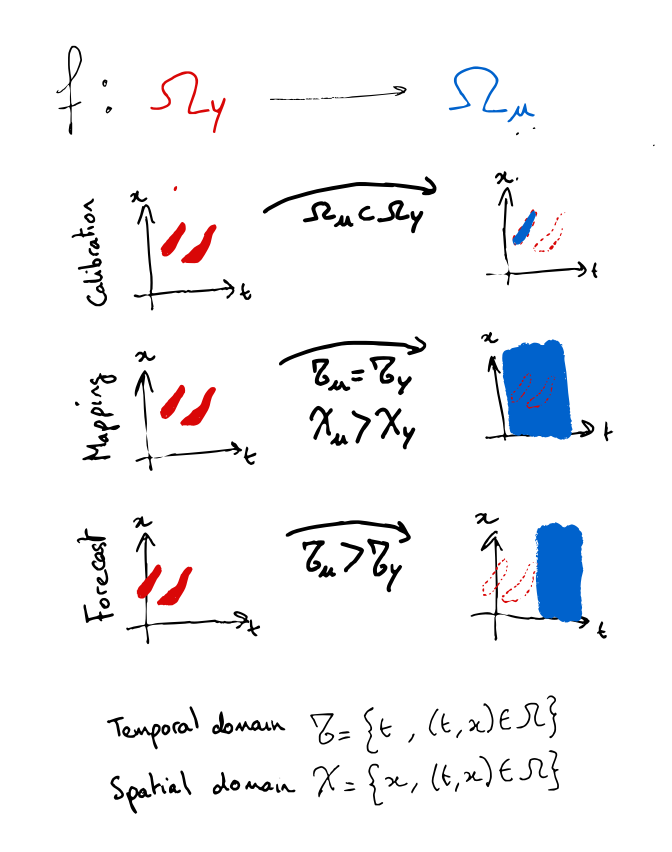
\includegraphics[width=0.8\linewidth]{Chapitre1/Ch1-Figures/Task_ontology.png} \\
   \end{center}
   \caption[Task characterization through the domains $\Omega_u$ and $\Omega_y$ of $u$ and $y$]
     {\footnotesize Using the perspective provided by the problem definition we can easily categorize earth observation problems.
     The calibration consist of estimating the field $u$ on a subset of the observation domain, the mapping consist in estimating $u$ on the same temporal domain but extending the spatial domain.
     And finally forecast can considered as wanting to estimate a quantity on an unobserved future domain.
   \label{fig:task_ontology}
\end{figure}

\section{Method Ontology}
  We're interested in characterizing and organizing the different methods that are used to tackle the class of problem introduced in \ref{sec:chap1_problem_form}.
  We postulate that all methods can be decomposed as the following two steps: 
  \begin{itemize}
    \item Step 1: Defining the set $\cal{F}$ of possible $f$ using theoritical knowledge (conceptual models)
    \item Step 2: Searching $\cal{F}$ for an optimal $f$ using factual knowledge (data)
  \end{itemize}

Let's walk through a simple example to illustrate our point, let's say we build a thermometer by putting a liquid in a tube and want to interpret the level of the thermometer as a temperature.
 As per our previous notations, $y$ is the level of the liquid and $u$ is the temperature of the liquid inside and we want to find the mapping $f$ between the two.

  The first step consists in compiling our theoritical knowledge on the problem to define the class of function. Given what we know on the fluid dilation with regard to temperature, under the assumption that the diameter of the tube is constant with height we can state that the level is linearly correlated with the temperature and therefore that $f$ will be part of $\cal{F} = \{ y: \alpha y + \beta , (\alpha, \beta) \in |R^2 \}$.
In order to find $\alpha$ and $\beta$, we move to step 2 where we need two datapoints to calibrate our model which would traditionally be obtained by putting the thermometer in icy and boiling water at 1 bar of pressure to get the levels corresponding to 0°C and 100°C.
  This method rely on strong theoritical basis and assumptions to reduce the dimensionality of the search space $\cal{F}$ and facilitate the parameter search using relatively few data points.

Now if we clearly see that the diameter of our thermometer is not constant. The model needs to incorporate that the evolution of the temperature depends on the diameter at each height. This expand the class of functions with a necessity to incorporate a model of the evolution of the diameter with in function of the height, which will introduce new parameters. We could for example assume the diameter is linear per part for every 5mm section and the corresponding parameters to search would be the value of the diameter every 5mm.

  In order to estimate these new parameters, we need more data which could be direct measures of the diameter or measures of temperature every 5mm.
  We could directly model $f$ as linear per part and therefore reduce the number of parameters to estimate (no more $\alpha$ and $\beta$). If we have measurements of the temperature, this also alleviate the need to explicitely model the relation between diameter and temperature.






  
% Tasks
% Simple exemple
% Calibration and mapping example

% Tasks of interests can be summed up as finding f
% Finding f takes two steps: defining the set of possible fs, searching the set for the best f
% Formulating the sets of F requires theoritical knowledge
% Searching the sets of F requires data

% From theory to sets of 
%   inverse problems state x
%   data assimilation: dynamical model
%   spatio temporal correlation: Covariance model
%   deep learning
%   locality: convolution
%   temporal dependence RNN LSTM


Lorem ipsum dolor sit amet, consectetuer adipiscing elit. Maecenas fermentum, elit non lobortis cursus, orci velit suscipit est, id mollis turpis mi eget orci.

\section{Première section du chapitre}

Lorem ipsum dolor sit amet, consectetuer adipiscing elit. Maecenas fermentum, elit non lobortis cursus, orci velit suscipit est, id mollis turpis mi eget orci.

\subsection{Première sous-section}

Lorem ipsum dolor sit amet, consectetuer adipiscing elit. Maecenas fermentum, elit non lobortis cursus, orci velit suscipit est, id mollis turpis mi eget orci.

Voir figure \ref{fig:mafigure2}.


\begin{figure}[htbp]
   \begin{center}
      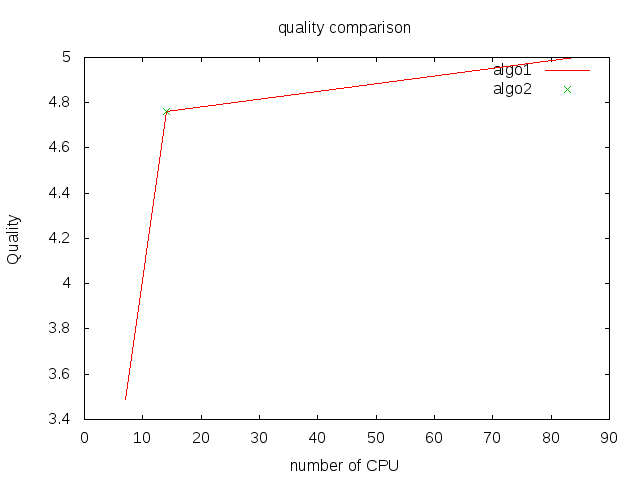
\includegraphics[width=0.8\linewidth]{Chapitre1/Ch1-Figures/comparison.png}
   \end{center}
   \caption[titre court pour la liste des figures]
   {\footnotesize Titre plus long avec des explications.}
   \label{fig:mafigure2}
\end{figure}

\subsection{Deuxième sous-section}

Lorem ipsum dolor sit amet, consectetuer adipiscing elit. Maecenas fermentum, elit non lobortis cursus, orci velit suscipit est, id mollis turpis mi eget orci.

\section{Conclusion du premier chapitre}

Lorem ipsum dolor sit amet, consectetuer adipiscing elit. Maecenas fermentum, elit non lobortis cursus, orci velit suscipit est, id mollis turpis mi eget orci.

In this manuscript I'd like to cite \cite{remo3,remo4}.

\addcontentsline{toc}{section}{Bibliography}
\putbib[./Chapitre1/Ch1-Biblio.bib]
\end{bibunit}
